\documentclass{article}
\usepackage[a4paper,margin=1in]{geometry}
\usepackage{amsmath, amsfonts, amssymb, amstext, mathtools, stmaryrd, textcomp, xcolor, graphicx, tikz}
\usepackage[hidelinks]{hyperref}
\usetikzlibrary{automata, positioning, arrows}
\tikzset{->,>=stealth,
every state/.style={thick, fill=gray!10}, 
initial text=$ $,
}
\newcommand{\e}{\varepsilon}
\newcommand{\s}{\Sigma}
\newcommand{\g}{\Gamma}
\newcommand{\so}{\rightarrow}
\newcommand{\str}{\texttt}
\newcommand{\newp}{\\[2mm]}
\newcommand{\defeq}{\coloneqq}

\title{Homework 03}
\author{Aaron Wang}
\date{February 17 2025}

\begin{document}
\maketitle
\begin{enumerate}
    \item \textbf{Regular expressions vs. Unix regular expressions.} Regular expressions and Unix regular expressions have some superficial differences, but also some deeper ones that affect the class of languages recognized.
    \begin{enumerate}
        \item Unix regular expressions have quantifiers: if $\alpha$ is a regular expression, $\alpha^{\{m,n\}}$ is a regular expression that matches at least $m$ and no more than $n$ strings that match $\alpha$. More formally, it matches all strings $w^{(1)}\cdots w^{(l)}$ where $m \leq l \leq n$, and for all $i$ such that $1 \leq i \leq l$, $w^{(i)}$ matches $\alpha$. Prove that for any regular expression with quantifiers, there is an equivalent regular expression without quantifiers.\newp
        \begin{figure}[ht]
\centering
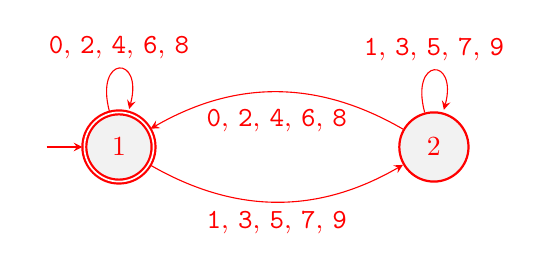
\begin{tikzpicture}
\color{red}
    \node[state, initial, accepting] (q1) {1};
    \node[state, right of=q1, xshift=3cm] (q2) {2};
    \draw (q1) edge[loop above] node[]{\str{0}, \str{2}, \str{4}, \str{6}, \str{8}} (q1)
    (q2) edge[loop above] node[]{\str{1}, \str{3}, \str{5}, \str{7}, \str{9}} (q2)
    (q2) edge[bend right] node[below, yshift=-0.1cm]{\str{0}, \str{2}, \str{4}, \str{6}, \str{8}} (q1)
    (q1) edge[bend right] node[below]{\str{1}, \str{3}, \str{5}, \str{7}, \str{9}} (q2);
\end{tikzpicture}
\end{figure}
        \item Unix regular expressions have backreferences: for an explanation, please see 
        \begin{center}
            \url{http://www.regular-expressions.info/backref.html}.
        \end{center} Give an example of a Unix regular expression that uses backreferences to describe a nonregular language, and prove that this language is not regular. We want you to get practice writing a non-regularity proof, so although you may use Examples 1.73–77, do not simply cite one of them; please write out a full proof. \newp
        \begin{figure}[ht]
\centering
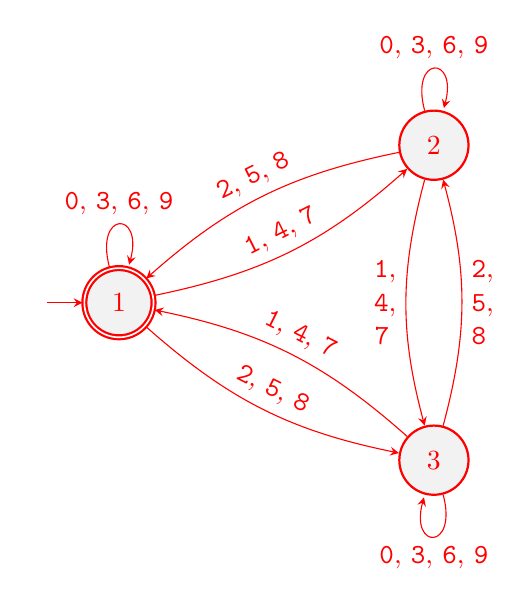
\begin{tikzpicture}
\color{red}
    \node[state, initial, accepting] (q1) {1};
    \node[state, right of=q1, xshift=3cm, yshift=2cm] (q2) {2};
    \node[state, right of=q1, xshift=3cm, yshift=-2cm]  (q3) {3};
% go forward one node  
    \draw (q1) edge[bend right=15] node[sloped, above]{\str{1}, \str{4}, \str{7}} (q2)
    (q2) edge[bend right=15] node[left, align=center]{\str{1},\\ \str{4},\\ \str{7}\:} (q3)
    (q3) edge[bend right=15] node[sloped, above]{\str{1}, \str{4}, \str{7}} (q1)
% go back one node     
    (q1) edge[bend right=15] node[sloped, above]{\str{2}, \str{5}, \str{8}} (q3)
    (q3) edge[bend right=15] node[right, align=center]{\str{2},\\ \str{5},\\ \str{8}\;} (q2)
    (q2) edge[bend right=15] node[sloped, above]{\str{2}, \str{5}, \str{8}} (q1)
% looping nodes
    (q1) edge[loop above] node[above]{\str{0}, \str{3}, \str{6}, \str{9}} (q1)
    (q2) edge[loop above] node[above]{\str{0}, \str{3}, \str{6}, \str{9}} (q2)
    (q3) edge[loop below] node[below]{\str{0}, \str{3}, \str{6}, \str{9}} (q3)
    ;     
\end{tikzpicture}
\end{figure}
    \end{enumerate}
\newpage
    \item \textbf{Binary addition.} This problem is about two ways of representating addition of binary natural numbers. We consider 0 to be a natural number. We allow binary representations of natural numbers to have leading 0s, and we consider $\e$ to be a binary representation of 0. When adding numbers, we do not allow overflow, so, for example, $1111 + 0001 = 0000$ is false.
    \begin{enumerate}
        \item [(a)] [Problem 1.32] Let
        \[
        \Sigma_3 = \left\{
        \begin{bmatrix}
        \str{0} \\ \str{0} \\ \str{0}
        \end{bmatrix},
        \begin{bmatrix}
        \str{0} \\ \str{0} \\ \str{1}
        \end{bmatrix},
        \begin{bmatrix}
        \str{0} \\ \str{1} \\ \str{0}
        \end{bmatrix},
        \begin{bmatrix}
        \str{0} \\ \str{1} \\ \str{1}
        \end{bmatrix},
        \begin{bmatrix}
        \str{1} \\ \str{0} \\ \str{0}
        \end{bmatrix},
        \begin{bmatrix}
        \str{1} \\ \str{0} \\ \str{1}
        \end{bmatrix},
        \begin{bmatrix}
        \str{1} \\ \str{1} \\ \str{0}
        \end{bmatrix},
        \begin{bmatrix}
        \str{1} \\ \str{1} \\ \str{1}
        \end{bmatrix}
        \right\},
        \]
        that is, an alphabet of eight symbols, each of which is a column of three bits. Thus, a string over $\s_3$ gives three rows of bits. Show that the following is regular: 
        \[
            B = \{w \in \s_3^* | \text{ the bottom row of w is the sum of the top two rows} \}.
        \]
        For example, because 011+001 = 100,
        \[
        \begin{bmatrix}
        \str{0} \\ \str{0} \\ \str{1}
        \end{bmatrix}
        \begin{bmatrix}
        \str{1} \\ \str{0} \\ \str{0}
        \end{bmatrix}
        \begin{bmatrix}
        \str{1} \\ \str{1} \\ \str{0}
        \end{bmatrix}
        \in B
        \]
        Hint: Since it’s easier to think about addition from right to left, design an automaton for $B^R$ first, then convert it into an automaton for $B$.\newp
        \begin{figure}[h]
\centering
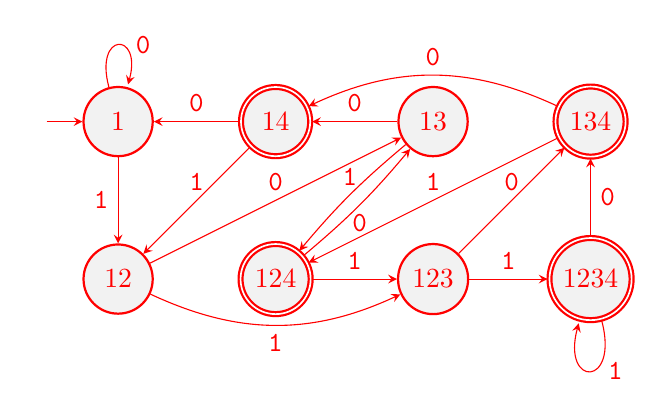
\begin{tikzpicture}
\color{red}
    % \node[state, initial] (q000) {$q_{000}$};
    % \node[state, yshift=-2cm] (q001) {$q_{001}$};
    % \node[state, xshift=4cm] (q010) {$q_{010}$};
    % \node[state, yshift=-2cm, xshift=4cm] (q011) {$q_{011}$};
    % \node[state, xshift=2cm, accepting] (q100) {$q_{100}$};
    % \node[state, yshift=-2cm, xshift=2cm, accepting] (q101) {$q_{101}$};
    % \node[state, xshift=6cm, accepting] (q110) {$q_{110}$};
    % \node[state, yshift=-2cm, xshift=6cm, accepting] (q111) {$q_{111}$};
    \node[state, initial] (q000) {1};
    \node[state, yshift=-2cm] (q001) {12};
    \node[state, xshift=4cm] (q010) {13};
    \node[state, yshift=-2cm, xshift=4cm] (q011) {123};
    \node[state, xshift=2cm, accepting] (q100) {14};
    \node[state, yshift=-2cm, xshift=2cm, accepting] (q101) {124};
    \node[state, xshift=6cm, accepting] (q110) {134};
    \node[state, yshift=-2cm, xshift=6cm, accepting] (q111) {1234};
    \draw 
        (q000) edge[loop above] node[right, xshift=1mm]{\str{0}} (q000)
        (q000) edge[] node[left]{\str{1}} (q001)
        (q001) edge[] node[above]{\str{0}} (q010)
        (q001) edge[bend right=25] node[below]{\str{1}} (q011)
        (q100) edge[] node[above]{\str{0}} (q000)
        (q100) edge[] node[above]{\str{1}} (q001)
        (q101) edge[bend right=5] node[below]{\str{0}} (q010)
        (q101) edge[] node[above]{\str{1}} (q011)
        (q010) edge[] node[above]{\str{0}} (q100)
        (q010) edge[bend right=5] node[above]{\str{1}} (q101)
        (q011) edge[] node[above]{\str{0}} (q110)
        (q011) edge[] node[above]{\str{1}} (q111)
        (q110) edge[bend right=25] node[above]{\str{0}} (q100)
        (q110) edge[] node[above]{\str{1}} (q101)
        (q111) edge[] node[right]{\str{0}} (q110)
        (q111) edge[loop below] node[right, xshift=1mm]{\str{1}} (q111)
    ;
\end{tikzpicture}
\end{figure}
        \item [(b)][Problem 1.53] Let $\s = \{\str{0}, \str{1}, +, =\}$, and prove that the following is not regular:
        \[
         ADD = \{x = y+z | x,y,z \in \{\str{0},\str{1}\}^*\text{ and } x=y+z \text{ is true }\}.
        \]
        \answer{
    Run $TM_{L2}$ on $\langle TM_{L2} \rangle$. Assume towards a contradiction that $TM_{L2}$ is 10-compliant. Thus we will be at step 4 and simulate $TM_{L2}$ on $\langle TM_{L2} \rangle$. This should either accept or reject.
    \begin{itemize}
        \item [] If $TM_{L2}$ accepts $\langle TM_{L2} \rangle$, then we must reject $\lightning$. 
        \item [] If $TM_{L2}$ rejects $\langle TM_{L2} \rangle$, then we must accept $\lightning$.
    \end{itemize}
    Since we have a contradiction, $TM_{L2}$ must not be 10-compliant.
}
    \end{enumerate}
\newpage
    \item \textbf{Similar but different} [Problem 1.49].
    \begin{enumerate}
        \item Let $B = \{\str{1}^kw | w \in\{\str{0}, \str{1}\}^* \text{ and $w$ contains at least $k$ 1s, for } k \geq 1 \}$. Show that $B$ is a regular language. Hint: Try out some strings to see what does and doesn’t belong to $B$, in order to find another simpler way of thinking about $B$.\newp
        \textcolor{red}{
The following is an NFA for B. The Intuition is this. First let's consider $k=1$. In this case, all we need is a $w$ that contains one \str{1}. Now consider, what if we thought $k$ was 2 or $s=\str{1}^2w$. Let us rewrite it as $s=\str{1}w'$ s.t. $w'=\str{1}w$. Now we have the same case as before. For any $k > 1$, we could do this such that $s=\str{1}^kw=\str{1}^1w'$ s.t. $w' = \str{1}^{k-1}w$. In essence, we now realize that we are looking only for a string that starts with \str{1} and contains at least 2 \str{1}s.
}
\begin{figure}[h]
\centering
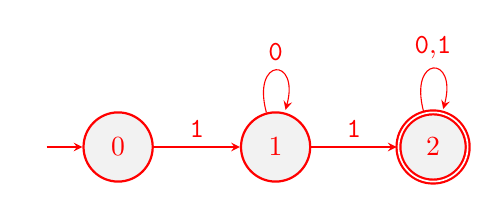
\begin{tikzpicture}
\color{red}
    \node[state, initial] (q0) {0};
    \node[state, xshift=2cm] (q1) {1};
    \node[state, xshift=4cm, accepting] (q2) {2};

    \draw
    (q0) edge[] node[above]{\str{1}} (q1)
    (q1) edge[loop above] node[above]{\str{0}} (q1)
    (q1) edge[] node[above]{\str{1}} (q2)
    (q2) edge[loop above] node[above]{\str{0},\str{1}} (q2)
    ;
\end{tikzpicture}
\end{figure}
        \item Let $C = \{\str{1}^kw | w \in\{\str{0}, \str{1}\}^* \text{ and $w$ contains at most $k$ 1s, for } k \geq 1 \}$. Prove that $C$ is not a regular language.\newp
        \textcolor{red}{
Let $M'$ be the Turing machine that describes STRETCH$(L)$\newp
$M' = $ ``On input string $w$''
\begin{quote}
\begin{enumerate}
    \item[1.] Simulate S
    \item[2.] If $S$ rejects $w$: \emph{reject}.
    \item[3.] If $S$ accepts $w$: Move head to start of tape\footnote{In the case that this is too high level, what one could do is add a preprocessing step, Mark the first two symbols, Run S, and then at this point rewind to marked symbol, unmark it and continue.} and simulate M on the current tape.
    \item[4.] \emph{accept} or \emph{reject} as $M$ would.
\end{enumerate}
\end{quote}
}
    \end{enumerate}
\end{enumerate}
\end{document}